% Created by tikzDevice version 0.10.1 on 2016-06-15 19:48:02
% !TEX encoding = UTF-8 Unicode
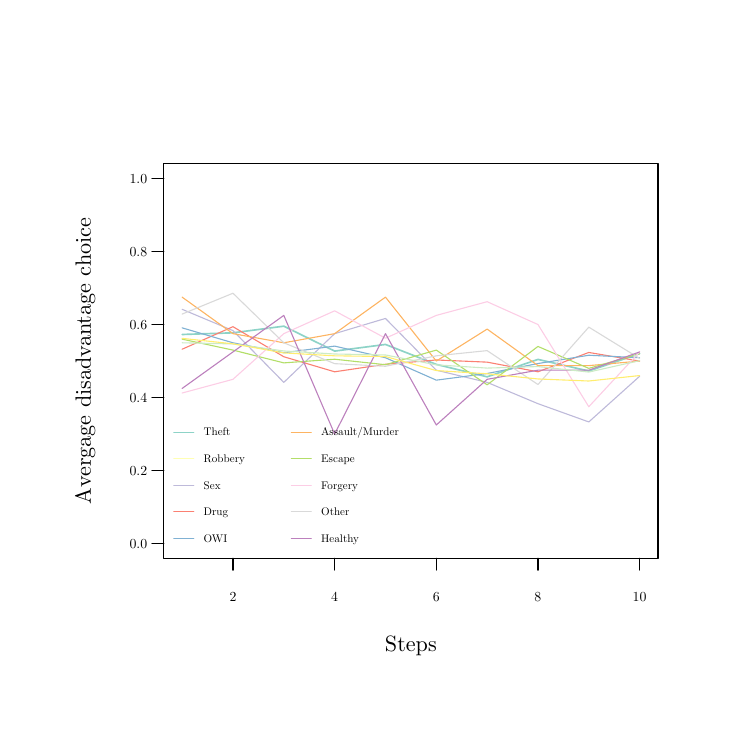
\begin{tikzpicture}[x=1pt,y=1pt]
\definecolor{fillColor}{RGB}{255,255,255}
\path[use as bounding box,fill=fillColor,fill opacity=0.00] (0,0) rectangle (252.94,252.94);
\begin{scope}
\path[clip] ( 49.20, 61.20) rectangle (227.75,203.75);
\definecolor{drawColor}{RGB}{141,211,199}

\path[draw=drawColor,line width= 0.6pt,line join=round,line cap=round] ( 55.81,142.07) --
	( 74.18,142.67) --
	( 92.55,145.07) --
	(110.92,136.07) --
	(129.29,138.47) --
	(147.66,131.27) --
	(166.03,126.77) --
	(184.39,133.07) --
	(202.76,128.87) --
	(221.13,135.17);
\end{scope}
\begin{scope}
\path[clip] (  0.00,  0.00) rectangle (252.94,252.94);
\definecolor{drawColor}{RGB}{0,0,0}

\path[draw=drawColor,line width= 0.4pt,line join=round,line cap=round] ( 74.18, 61.20) -- (221.13, 61.20);

\path[draw=drawColor,line width= 0.4pt,line join=round,line cap=round] ( 74.18, 61.20) -- ( 74.18, 56.92);

\path[draw=drawColor,line width= 0.4pt,line join=round,line cap=round] (110.92, 61.20) -- (110.92, 56.92);

\path[draw=drawColor,line width= 0.4pt,line join=round,line cap=round] (147.66, 61.20) -- (147.66, 56.92);

\path[draw=drawColor,line width= 0.4pt,line join=round,line cap=round] (184.39, 61.20) -- (184.39, 56.92);

\path[draw=drawColor,line width= 0.4pt,line join=round,line cap=round] (221.13, 61.20) -- (221.13, 56.92);

\node[text=drawColor,anchor=base,inner sep=0pt, outer sep=0pt, scale=  0.50] at ( 74.18, 45.60) {2};

\node[text=drawColor,anchor=base,inner sep=0pt, outer sep=0pt, scale=  0.50] at (110.92, 45.60) {4};

\node[text=drawColor,anchor=base,inner sep=0pt, outer sep=0pt, scale=  0.50] at (147.66, 45.60) {6};

\node[text=drawColor,anchor=base,inner sep=0pt, outer sep=0pt, scale=  0.50] at (184.39, 45.60) {8};

\node[text=drawColor,anchor=base,inner sep=0pt, outer sep=0pt, scale=  0.50] at (221.13, 45.60) {10};

\path[draw=drawColor,line width= 0.4pt,line join=round,line cap=round] ( 49.20, 66.48) -- ( 49.20,198.47);

\path[draw=drawColor,line width= 0.4pt,line join=round,line cap=round] ( 49.20, 66.48) -- ( 44.92, 66.48);

\path[draw=drawColor,line width= 0.4pt,line join=round,line cap=round] ( 49.20, 92.88) -- ( 44.92, 92.88);

\path[draw=drawColor,line width= 0.4pt,line join=round,line cap=round] ( 49.20,119.27) -- ( 44.92,119.27);

\path[draw=drawColor,line width= 0.4pt,line join=round,line cap=round] ( 49.20,145.67) -- ( 44.92,145.67);

\path[draw=drawColor,line width= 0.4pt,line join=round,line cap=round] ( 49.20,172.07) -- ( 44.92,172.07);

\path[draw=drawColor,line width= 0.4pt,line join=round,line cap=round] ( 49.20,198.47) -- ( 44.92,198.47);

\node[text=drawColor,anchor=base east,inner sep=0pt, outer sep=0pt, scale=  0.50] at ( 43.20, 64.76) {0.0};

\node[text=drawColor,anchor=base east,inner sep=0pt, outer sep=0pt, scale=  0.50] at ( 43.20, 91.15) {0.2};

\node[text=drawColor,anchor=base east,inner sep=0pt, outer sep=0pt, scale=  0.50] at ( 43.20,117.55) {0.4};

\node[text=drawColor,anchor=base east,inner sep=0pt, outer sep=0pt, scale=  0.50] at ( 43.20,143.95) {0.6};

\node[text=drawColor,anchor=base east,inner sep=0pt, outer sep=0pt, scale=  0.50] at ( 43.20,170.35) {0.8};

\node[text=drawColor,anchor=base east,inner sep=0pt, outer sep=0pt, scale=  0.50] at ( 43.20,196.74) {1.0};

\path[draw=drawColor,line width= 0.4pt,line join=round,line cap=round] ( 49.20, 61.20) --
	(227.75, 61.20) --
	(227.75,203.75) --
	( 49.20,203.75) --
	( 49.20, 61.20);
\end{scope}
\begin{scope}
\path[clip] (  0.00,  0.00) rectangle (252.94,252.94);
\definecolor{drawColor}{RGB}{0,0,0}

\node[text=drawColor,anchor=base,inner sep=0pt, outer sep=0pt, scale=  0.80] at (138.47, 27.60) {Steps};

\node[text=drawColor,rotate= 90.00,anchor=base,inner sep=0pt, outer sep=0pt, scale=  0.80] at ( 22.80,132.47) {Avergage disadvantage choice};
\end{scope}
\begin{scope}
\path[clip] ( 49.20, 61.20) rectangle (227.75,203.75);
\definecolor{drawColor}{RGB}{190,186,218}

\path[draw=drawColor,line width= 0.4pt,line join=round,line cap=round] ( 55.81,151.17) --
	( 74.18,143.47) --
	( 92.55,124.77) --
	(110.92,142.37) --
	(129.29,147.87) --
	(147.66,129.17) --
	(166.03,124.77) --
	(184.39,117.07) --
	(202.76,110.47) --
	(221.13,126.97);
\definecolor{drawColor}{RGB}{251,128,114}

\path[draw=drawColor,line width= 0.4pt,line join=round,line cap=round] ( 55.81,136.74) --
	( 74.18,144.89) --
	( 92.55,134.03) --
	(110.92,128.59) --
	(129.29,131.31) --
	(147.66,132.86) --
	(166.03,132.08) --
	(184.39,128.59) --
	(202.76,135.58) --
	(221.13,132.47);
\definecolor{drawColor}{RGB}{128,177,211}

\path[draw=drawColor,line width= 0.4pt,line join=round,line cap=round] ( 55.81,144.47) --
	( 74.18,139.07) --
	( 92.55,135.47) --
	(110.92,137.87) --
	(129.29,133.67) --
	(147.66,125.57) --
	(166.03,127.97) --
	(184.39,131.57) --
	(202.76,134.57) --
	(221.13,133.67);
\definecolor{drawColor}{RGB}{253,180,98}

\path[draw=drawColor,line width= 0.4pt,line join=round,line cap=round] ( 55.81,155.57) --
	( 74.18,142.37) --
	( 92.55,139.07) --
	(110.92,142.37) --
	(129.29,155.57) --
	(147.66,132.47) --
	(166.03,144.02) --
	(184.39,130.82) --
	(202.76,130.82) --
	(221.13,132.47);
\definecolor{drawColor}{RGB}{179,222,105}

\path[draw=drawColor,line width= 0.4pt,line join=round,line cap=round] ( 55.81,140.39) --
	( 74.18,136.43) --
	( 92.55,131.81) --
	(110.92,133.13) --
	(129.29,131.15) --
	(147.66,136.43) --
	(166.03,123.89) --
	(184.39,137.75) --
	(202.76,129.83) --
	(221.13,135.11);
\definecolor{drawColor}{RGB}{252,205,229}

\path[draw=drawColor,line width= 0.4pt,line join=round,line cap=round] ( 55.81,120.92) --
	( 74.18,125.87) --
	( 92.55,142.37) --
	(110.92,150.62) --
	(129.29,140.72) --
	(147.66,148.97) --
	(166.03,153.92) --
	(184.39,145.67) --
	(202.76,115.97) --
	(221.13,135.77);
\definecolor{drawColor}{gray}{0.85}

\path[draw=drawColor,line width= 0.4pt,line join=round,line cap=round] ( 55.81,149.44) --
	( 74.18,156.98) --
	( 92.55,139.07) --
	(110.92,131.53) --
	(129.29,130.59) --
	(147.66,134.36) --
	(166.03,136.24) --
	(184.39,123.99) --
	(202.76,144.73) --
	(221.13,133.42);
\definecolor{drawColor}{RGB}{188,128,189}

\path[draw=drawColor,line width= 0.4pt,line join=round,line cap=round] ( 55.81,122.57) --
	( 74.18,135.77) --
	( 92.55,148.97) --
	(110.92,106.08) --
	(129.29,142.37) --
	(147.66,109.37) --
	(166.03,125.87) --
	(184.39,129.17) --
	(202.76,129.17) --
	(221.13,135.77);
\definecolor{drawColor}{RGB}{204,235,197}

\path[draw=drawColor,line width= 0.4pt,line join=round,line cap=round] ( 55.81,139.07) --
	( 74.18,138.66) --
	( 92.55,136.12) --
	(110.92,135.02) --
	(129.29,134.67) --
	(147.66,131.10) --
	(166.03,129.93) --
	(184.39,130.48) --
	(202.76,128.49) --
	(221.13,132.61);
\definecolor{drawColor}{RGB}{255,237,111}

\path[draw=drawColor,line width= 0.4pt,line join=round,line cap=round] ( 55.81,140.67) --
	( 74.18,138.70) --
	( 92.55,135.42) --
	(110.92,134.36) --
	(129.29,134.11) --
	(147.66,129.03) --
	(166.03,127.88) --
	(184.39,126.00) --
	(202.76,125.26) --
	(221.13,127.23);
\definecolor{drawColor}{RGB}{141,211,199}

\path[draw=drawColor,line width= 0.4pt,line join=round,line cap=round] ( 52.80,106.80) -- ( 60.00,106.80);
\definecolor{drawColor}{RGB}{255,255,179}

\path[draw=drawColor,line width= 0.4pt,line join=round,line cap=round] ( 52.80, 97.20) -- ( 60.00, 97.20);
\definecolor{drawColor}{RGB}{190,186,218}

\path[draw=drawColor,line width= 0.4pt,line join=round,line cap=round] ( 52.80, 87.60) -- ( 60.00, 87.60);
\definecolor{drawColor}{RGB}{251,128,114}

\path[draw=drawColor,line width= 0.4pt,line join=round,line cap=round] ( 52.80, 78.00) -- ( 60.00, 78.00);
\definecolor{drawColor}{RGB}{128,177,211}

\path[draw=drawColor,line width= 0.4pt,line join=round,line cap=round] ( 52.80, 68.40) -- ( 60.00, 68.40);
\definecolor{drawColor}{RGB}{253,180,98}

\path[draw=drawColor,line width= 0.4pt,line join=round,line cap=round] ( 95.26,106.80) -- (102.46,106.80);
\definecolor{drawColor}{RGB}{179,222,105}

\path[draw=drawColor,line width= 0.4pt,line join=round,line cap=round] ( 95.26, 97.20) -- (102.46, 97.20);
\definecolor{drawColor}{RGB}{252,205,229}

\path[draw=drawColor,line width= 0.4pt,line join=round,line cap=round] ( 95.26, 87.60) -- (102.46, 87.60);
\definecolor{drawColor}{gray}{0.85}

\path[draw=drawColor,line width= 0.4pt,line join=round,line cap=round] ( 95.26, 78.00) -- (102.46, 78.00);
\definecolor{drawColor}{RGB}{188,128,189}

\path[draw=drawColor,line width= 0.4pt,line join=round,line cap=round] ( 95.26, 68.40) -- (102.46, 68.40);
\definecolor{drawColor}{RGB}{0,0,0}

\node[text=drawColor,anchor=base west,inner sep=0pt, outer sep=0pt, scale=  0.40] at ( 63.60,105.42) {Theft};

\node[text=drawColor,anchor=base west,inner sep=0pt, outer sep=0pt, scale=  0.40] at ( 63.60, 95.82) {Robbery};

\node[text=drawColor,anchor=base west,inner sep=0pt, outer sep=0pt, scale=  0.40] at ( 63.60, 86.22) {Sex};

\node[text=drawColor,anchor=base west,inner sep=0pt, outer sep=0pt, scale=  0.40] at ( 63.60, 76.62) {Drug};

\node[text=drawColor,anchor=base west,inner sep=0pt, outer sep=0pt, scale=  0.40] at ( 63.60, 67.02) {OWI};

\node[text=drawColor,anchor=base west,inner sep=0pt, outer sep=0pt, scale=  0.40] at (106.06,105.42) {Assault/Murder};

\node[text=drawColor,anchor=base west,inner sep=0pt, outer sep=0pt, scale=  0.40] at (106.06, 95.82) {Escape};

\node[text=drawColor,anchor=base west,inner sep=0pt, outer sep=0pt, scale=  0.40] at (106.06, 86.22) {Forgery};

\node[text=drawColor,anchor=base west,inner sep=0pt, outer sep=0pt, scale=  0.40] at (106.06, 76.62) {Other};

\node[text=drawColor,anchor=base west,inner sep=0pt, outer sep=0pt, scale=  0.40] at (106.06, 67.02) {Healthy};
\end{scope}
\end{tikzpicture}
